\documentclass[12pt]{article}

% Set the page to be letter paper and have small margins
\usepackage{geometry}
\geometry{letterpaper, left=15mm, right=15mm, top=15mm, bottom=20mm}

% LuaLaTeX font setup
\usepackage{fontspec}
\usepackage{unicode-math}

% Text font
\setmainfont{DejaVu Serif}

% Math font
\setmathfont{STIX Two Math}

\allowdisplaybreaks[1]

\usepackage{standalone}
\usepackage{parskip}
\usepackage{amsmath}
\usepackage{amsthm}
\usepackage{multicol}
\usepackage{graphicx}
\usepackage{pgfplots}
\pgfplotsset{compat=1.18}
\usepackage{cancel}
\usepackage{xcolor}
\usepackage[utf8]{inputenc}
\usepackage{float}
\usepackage{graphicx}
\usepackage{pdfpages}
\usepackage{booktabs}

% \usepackage{hyperref}
\usepackage{cleveref}


\usepackage{titlesec}
\titleformat{\section}{\normalfont\normalsize\bfseries}{\thesection.}{1em}{}
\titleformat{\subsection}{\normalfont\normalsize\bfseries\itshape}{\thesubsection}{1em}{}

\usepackage{enumitem}
\setlist[enumerate, 1]{label=\textbf{\arabic*}.}
\setlist[enumerate, 2]{label=\textbf{\alph*}.}

% \usepackage[style=ieee]{biblatex}
% \addbibresource{src/refs.bib}

\makeatletter
\newcommand{\course}[1]{\def\@course{#1}}

\renewcommand{\maketitle}{
    \noindent
    \@author \hfill \@course \newline
    \@date
    \begin{center}
        \large\textbf{\@title}
    \end{center}
    \bigskip
}

\author{Jeffrey Morris}
\course{MATH 4306-010}
\date{\today}


\begin{document}
\begin{center}
    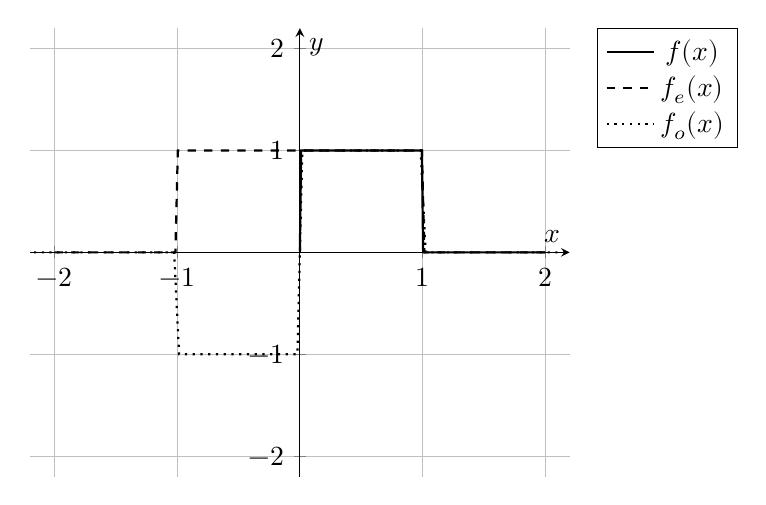
\begin{tikzpicture}
        \begin{axis}[
                axis lines=middle,
                grid=both,
                xmin=-2.2, xmax=2.2,
                ymin=-2.2, ymax=2.2,
                samples=200,
                xlabel={$x$},
                ylabel={$y$},
                legend style={at={(1.05,1)},anchor=north west}
            ]

            \addplot[thick,domain=0:2]{ ( x>0 && x<1) ? 1 : 0};
            \addlegendentry{$f(x)$}

            \addplot[thick,domain=-2:2,dashed] { (abs(x)>0 && abs(x)<1) ? 1 : 0};
            \addlegendentry{$f_e(x)$}

            \addplot[thick,domain=-4:4,dotted] { (abs(x)>0 && abs(x)<1) ? sign(x) : 0};
            \addlegendentry{$f_o(x)$}

        \end{axis}
    \end{tikzpicture}
\end{center}
\begin{align*}
    f_c(x)     & =\frac{2}{\pi} \int_{0}^{\infty}A(\lambda)\cos(\lambda x)\,d\lambda                           \\
    A(\lambda) & =\int_{0}^{\infty}f(x)\cos(\lambda x)\,dx                                                     \\
    A(\lambda) & =\int_{0}^{1}\cos(\lambda x)\,dx                                                              \\
    A(\lambda) & =\frac{1}{\lambda} \left[ \sin(\lambda x) \right]_0^1                                         \\
    A(\lambda) & =\frac{1}{\lambda} \left[ \sin(\lambda) - \cancelto{0}{\sin(0)} \right]                       \\
    A(\lambda) & =\frac{\sin(\lambda)}{\lambda}                                                                \\
    f_c(x)     & = \boxed{\frac{2}{\pi}\int_{0}^{\infty}\frac{sin(\lambda)}{\lambda}\cos(\lambda x)\,d\lambda} \\
\end{align*}
\begin{align*}
    f_s(x)     & = \frac{2}{\pi} \int_{0}^{\infty} B(\lambda)\sin(\lambda x)\,d\lambda                                         \\
    B(\lambda) & = \int_{0}^{\infty} f(x)\sin(\lambda x)\,dx                                                                   \\
    B(\lambda) & = \int_{0}^{1} \sin(\lambda x)\,dx                                                                            \\
    B(\lambda) & = \frac{-1}{\lambda} \left[ \cos(\lambda x) \right]_0^1                                                       \\
    B(\lambda) & = \frac{-1}{\lambda} \left[ \cos(\lambda) - \cancelto{1}{\cos(0)} \right]                                     \\
    B(\lambda) & = \frac{-1}{\lambda} \left[ \cos(\lambda) - 1 \right]                                                         \\
    f_s(x)     & = \boxed{\frac{2}{\pi} \int_{0}^{\infty} \frac{sin(\lambda x)}{\lambda} \left[ 1 - \cos(\lambda) \right]\,dy}
\end{align*}
\end{document}